%First, make the design space as large as possible
% tradeoffs/considerations/selection
% 1 or 2 solutions

First, let us list the design decisions. The first design decision is how to encode explicit datapaths such that the hardware knows about bypasses. Then there is the manner of when in the compilation chain does it actually encode these bypasses.
%TODO: extend with other decisions that are added below.

%TODO: add decision of how to encode the bypass registers. Choice to use register index space or add bits to instruction

%TODO: (is explained at class diagram 3.4.3) add decision for predicate flag instructions, we made getStartOperand to skip flagged instructions. Alternatively, it is also possible to ignore any flag operands that are encountered.

\subsubsection{Encoding bypasses}
The first design decision is how to encode that an operand is forwarded. There are two ways to encode that a source operand comes from the bypass network:
\begin{figure}[b!]
\centering
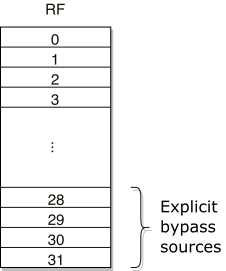
\includegraphics[width=.225\textwidth]{figures/encoding}
\caption{Illustration of reserving a portion of the register index space to encode explicit datapaths.}
\label{fig:rf_index_space}
\end{figure}

\begin{enumerate}[i.]
  \item Add bits to each instruction to specify that a certain operand comes from the bypass network. It requires three bits per source operands because there are five different bypass sources with a five-stage pipeline. Each instruction may have up to two source operands that can be bypassed. Therefore, this approach requires six additional bits to be added to each instruction.
  \item Use register index space to indicate that an operand comes from the bypass network. This requires at most five registers to be reserved because there are at most five bypass sources.
\end{enumerate} 

The approach in which the register index space is used to encode that an operand is bypassed was chosen because the hardware description of the architecture corresponds to that, and because this does not require any modification to the instruction format.

The other approach would be beneficial since it does not reduce the register file index space such that limitations to high register pressure can be avoided.

\begin{figure}[b!]
\centering
\subfloat[Explicit bypassing before RA.]{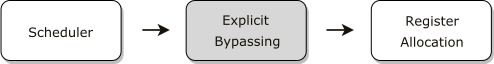
\includegraphics[width=.645\textwidth]{figures/explicit_bypass_allocationA}%
\label{fig:expl_bp_A}}
\vspace{10px}
\subfloat[Explicit bypassing after RA.]{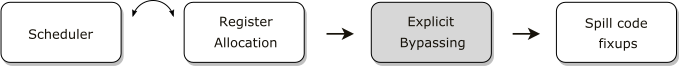
\includegraphics[width=.9\textwidth]{figures/explicit_bypass_allocationB}%
\label{fig:expl_bp_B}}
\caption{When to apply explicit bypasses.}
\label{fig:expl_bp}
\end{figure}

\subsubsection{When and how to allocate explicit bypasses}
When to actually do this can be categorized in three approaches. Trivially, it is not possible to do explicit bypass allocation before scheduling, because one needs a schedule to allocate explicit bypasses. %the order of instructions is not known at that time. 
(i) Ideally it would be done before register allocation (Figure \ref{fig:expl_bp_A}) where there are still virtual registers. The number of virtual registers reduces with each store that is avoided. Thereby, reducing register pressure and relaxing the job for the register allocator.

However, when the register allocator runs out of registers and inserts spill code between two instructions that were already bypassed, this bypass may not be valid anymore and may even require an additional register to undo that bypass.

(ii) Alternatively it can be done after register allocation. However, the physical registers that are freed by dead result elimination are not exploited when doing this after RA. Because, if spill code was necessary it has already been inserted during register allocation. Therefore, after the explicit bypasses have been allocated, the resulting assembly code may have redundant spill code and does not gain from reduced register pressure. With this approach it does not matter whether to do scheduling or RA first, which is illustrated in Figure \ref{fig:expl_bp_B}.

(iii) Finally, it is also possible to do scheduling and register allocation in one go with constraint programming. However, this problem is NP-complete and may take an unbounded amount of time. \\



%\begin{figure}[t]
%\centering
%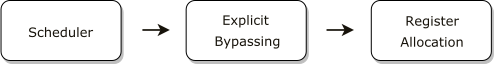
\includegraphics[width=.8\textwidth]{figures/explicit_bypass_allocation_A}
%\caption{Phase ordering problem.}
%\label{fig:expl_bp_A}
%\end{figure}

%\begin{figure}[b]
%\centering
%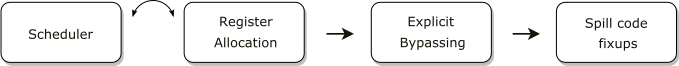
\includegraphics[width=.9\textwidth]{figures/explicit_bypass_allocation_B}
%\caption{Phase ordering problem.}
%\label{fig:expl_bp_B}
%\end{figure}

To summarize, ideally the explicit datapaths are exploited before register allocation to gain from reduced register pressure, but it is extremely difficult to insert spill code. So alternatively, it can be done after register allocation which may potentially have redundant spill code. For the later approach, an effort to clean up redundant spill code may be desired for more efficient code.\\

How to exploit explicit register allocation is a very broad question, in fact this is the main goal of this assignment. Let us split up in two categories of approaches:
\begin{enumerate}[i.]
  \item One way to exploit explicit datapaths is to group instructions close to their use. Moreover, if an instruction is strictly adjacent to its use, it may immediately be bypassed.%Group instructions together and allocate special bypass registers on the fly. Moreover, when this is done before register allocation where we have virtual registers, the number of virtual registers reduces with each bypass that we allocate. Thereby, reducing register pressure and relaxing the job for the register allocator.
  \item Another way to exploit explicit datapaths is by going through a basic block (a code sequence with no branches in except to the entry and no branches out except at the exit) and allocate explicit bypasses as a post-processing step, in the sense that this is done when the schedule does not change anymore.
\end{enumerate}

\begin{figure}[t]
\centering
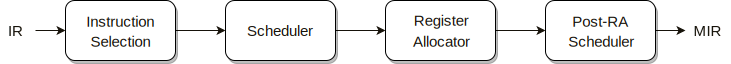
\includegraphics[width=.9\textwidth]{figures/phase_ordering}
\caption{Phase ordering problem.}
\label{fig:phase_ordering}
\end{figure}

The approach in the first category where instructions are grouped together has a problem. When a bypass is done early on, it needs to be verified if it is still valid after a change to the schedule has been made. In the compilation chain (Figure \ref{fig:phase_ordering}) the order in which instructions are executed is first decided by the general scheduler. The register allocator may insert spill code at any place in the schedule. After that, the order may change again by the post-RA scheduler or by a custom pass.\\

Now let us discuss the second approach that works on a basic block. The assumption in this approach is that the order in which instructions are executed is set and does not change anymore. Therefore, each bypass that is applied stays valid. 
%We can allocate explicit bypass register on an instruction if we have a RaW dependency between that instruction and an instruction in the pipeline state model.
The problem that remains is when there are multiple branches to the basic block. With multiple branches in, the state of the pipeline and which bypasses may be allocated can be different depending on which branch is taken. This problem is referred to as the join problem which is illustrated by example in Listing \ref{lst:join_problem}. Depending on which branch is taken the value of register \texttt{r7} may be forwarded from \texttt{ALU} when coming from \texttt{\%if}, or from \texttt{MUL} when coming from \texttt{\%else} which leads to an ambiguous pipeline state. Thus, the use of \texttt{r7} in \texttt{\%end} is forwarded from the bypass network, but is ambiguous and this together with being bypassed is not allowed for explicit datapaths. Therefore, such ambiguous behaviour should either be avoided or fixed, such that it is absent in the generated code.

\captionof{lstlisting}{Fragment of C code with corresponding assembly, to illustrate the join problem.}\label{lst:join_problem}
\begin{center}
\hspace{2px}\begin{minipage}{.475\textwidth}
\lstset{style=customc}
%\begin{lstlisting}[caption=List of instructions.,frame=tlrb]
\begin{lstlisting}[frame=tlrb]
int foo(int a, int b, int c)
{
  if (a > b)
    c += 5;
  else
    c = c * 3;
  c = c - a;
  return c;
}

<@\ @>
\end{lstlisting}
\end{minipage}\hfill
\begin{minipage}{.475\textwidth}
\lstset{style=customasm}
%\begin{lstlisting}[caption=IR-code.,frame=tlrb]
\begin{lstlisting}[frame=tlrb]
$foo:           # a = r5, b = r6 and c = r7
  sfles r5, r6
  bf    $else
  nop
$if:
  j     $end
  add   r7, r7, 5   # r7 in ALU
$else:
  mul   r7, r7, 3   # r7 in MUL 
$end:
  sub   r3, r7, r5  # r7 from MUL or ALU?
\end{lstlisting}
%\vspace{1.9em}
\end{minipage}
\end{center}

Bypassing with a limited scope of only a basic block requires multiple no-ops to be inserted on the end of each block, such that the pipeline state is flushed and no ambiguous behaviour occurs. Going from intra- to an inter basic block scope the ambiguous behaviour may be fixed using a technique which is discussed in the next section. With a function-level scope the pipeline state needs to be flushed only on a function call, because many instructions will be executed before returning. No-ops are not required because the prologue and epilogue insertions guarantee unambiguous behaviour between function calls. Going to a module-level scope would even allow bypasses from one function to another. However, because of time limitations, and because this only increases the bypasses with just a little bit, a module-level scope has not been implemented.\\

To conclude, the first approach discussed above may improve utilization of the bypass network, but can not be used as a stand-alone approach, since it does not solve the join problem. While the second approach works on a single basic block, it can easily be extended to a larger scope (for example, a function-level scope or a module-level scope). The following sections will show how the join problem can be tackled when a larger scope is considered. 

%When we bypass a value that is defined in another basic block, we require all blocks with a branch to that basic block to have that value in the same bypass source.

%REMOVE TEXT BELOW!!!
%We exploit explicit datapaths by going through a basic block (a code sequence with no branches in except to the entry and no branches out except at the exit) and allocate explicit bypass registers as a post-processing step, in the sense that we do this after scheduling, register allocation, packetizing, etc. Doing this as a post-processing step has advantages compared to doing this early on. 

%TODO: discuss add text below? ask Luc or Roel
%\begin{enumerate}[i.]
%\item When this is done after the packetizer it has bundled `VLIW' instructions consisting of both a scalar and a vector operation which reduces complexity of the bypassing approach.
%\item Another reason to do bypass allocation as a post-processing step is that doing it at an earlier stage, where the code is not certain yet, gives more problems. Each of the custom passes may reorder or insert instructions which may invalidate a bypass already allocated before that point.
%\end{enumerate}
%However, doing it early on also has an advantage.
%TODO: add problem with post-processing approach. Namely, doing this before register allocation reduces register pressure. RA tries to find a physical register for each virtual register. When we change some of these virtual registers with bypass registers already, we end do not need to find a physical register for these, thereby, reducing register pressure.

%clue


%TODO: continue writing xxx 
